\chapter{METODE PENELITIAN}

\noindent Dalam penelitian ini akan dilakukan implementasi model Attention U-net untuk segmentasi mikrovaskular dalam WSI ginjal manusia sehat.  Penggunaan \textit{Aattention Gate} (AG) pada U-net dipilih untuk memusatkan perhatian model pada \textit{feature} yang berpengaruh dari \textit{encoder} ,sehingga bisa meningkatkan peforma model dalam tugas segmentasi mikrovaskular dalam WSI ginjal manusia sehat. Penelitian ini melibatkan beberapa tahapan mulai dari penginputan data sampai ke evaluasi model. Secara mendetail seluruh proses dari penelitian ini bisa dilihat pada flowchart berikut ini:
\begin{figure}[H]
	\centering
	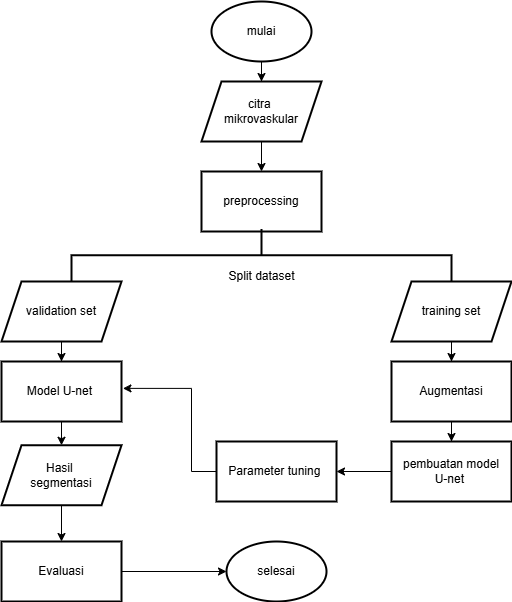
\includegraphics[scale=.6]{gambar/flow-chart.png}
	\caption{Flow chart Penerapan U-net}
	\label{fig:flow-chart}
\end{figure}

\section{Dataset Penelitian}

\noindent Dataset yang digunakan pada penelitian ini adalah data yang telah disediakan \textit{Human BioMolecular Atlas Program }(HuBMAP) di Kaggle: \url{https://www.kaggle.com/competitions/hubmap-organ-segmentation}\cite{howard_hubmap_2023}.  Data ini berisi citra WSL mikrovaskular ginjal manusia yang telah diwarnai menggunakan metode \textit{2D PAS-stained}. \textit{2D PAS-stained} mengacu pada citra dua dimensi yang diwarnai menggunakan pewarnaan Periodic Acid-Schiff (PAS). Data ini terdiri dari 7033 citra yang telah diwarnai dengan format TIFF beresolusi 512x512 dimana 1633 telah dianotasikan ke tiga kelas yakni, \textit{blood vessels}(pembuluh darah), \textit{glomelurus} dan \textit{unsure}(dikeragui).  Anotasi dari data tersebut disimpan dalam file json yang merepresentasikan kordinat mask poligon yang sesuai dengan area setiap kelas pada gambar. Dalam penelitian ini hanya data yang telah dianotasikan saja yang akan digunakan untuk melatih model dengan menggabungkan ketiga kelas anotasi menjadi satu kelas mikrovaskular.

\begin{figure}[H]
	\centering
	\begin{subfigure}[b]{0.3\textwidth}
		\centering
		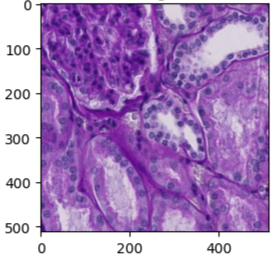
\includegraphics[width=\textwidth]{gambar/image.png}
		\caption{Image}
		\label{fig:image}
	\end{subfigure}
	\hfill
	\begin{subfigure}[b]{0.3\textwidth}
		\centering
		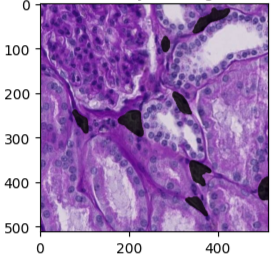
\includegraphics[width=\textwidth]{gambar/overlayed_image.png}
		\caption{Ovelayed image}
		\label{fig:overlayed-image}
	\end{subfigure}
	\hfill
	\begin{subfigure}[b]{0.3\textwidth}
		\centering
		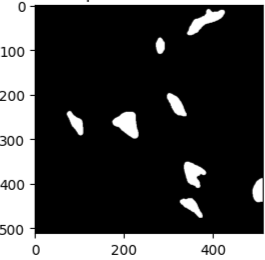
\includegraphics[width=\textwidth]{gambar/pixelwise_label.png}
		\caption{Pixel wise label}
		\label{fig:Pixel wise label}
	\end{subfigure}
	\caption{Sample WSI yang telah dianotasikan}
	\label{fig:sample_data}
\end{figure}

\section{Spesifikasi Perangkat}

\noindent Penelitian ini akan dilakukan di lingkungan komputasi remote menggunakan \textit{Kaggle Notebooks}. Kaggle menyediakan perangkat keras yang diperlukan dalam penelitian, sehingga peneliti bisa fokus pada eksekusi teori ke dalam kode python tanpa perlu konfigurasi perangkat terlebih dahulu. Spesifikasi sumber daya komputasi yang disediakan Kaggle bisa dilihat pada tabel \ref{tab:cpu_specs}.
\begin{table}[h]
	\centering
	\caption{Spesifikasi CPU pada Lingkungan Komputasi Remote Kaggle Notebook.} % caption pakai titik?
	\label{tab:cpu_specs}
	\begin{tabular}{lllll}
		\hline
		\textbf{Jenis} & \textbf{CPU}                             & \textbf{Core CPU} & \textbf{RAM} & \textbf{GPU}        \\ \hline
		CPU            & Default & 4                 & 30 GB        & -                   \\ \hline
		GPU P100       & Intel Skylake                            & 4                 & 29 GB        & 1 Nvidia Tesla P100 \\ \hline
		GPU T4 x2      & Intel Skylake                            & 4                 & 29 GB        & 2 Nvidia Tesla T4   \\ \hline
		TPU 1VM        & -                                        & 96                & 330 GB       & -                   \\ \hline
	\end{tabular}
\end{table}

\noindent \textit{Notebook} yang menggunakan \textit{Central Processing Unit }(CPU) dan \textit{Graphics Processing Unit} (GPU) memiliki waktu eksekusi selama 12 jam, sedangkan notebook yang menggunakan \textit{Tensor Processing Unit} (TPU) memiliki waktu eksekusi selama 9 jam. Tersedia 20 \textit{Gigabytes} ruang penyimpanan otomatis direktori '/kaggle/working' dan ruang penyimpanan \textit{scratchpad} tambahan yang tidak akan disimpan diluar sesi saat ini.


\section{Preproccessing}

\noindent \textit{Preproccessing} merupakan langkah penting dalam mempersiapkan dataset agar bisa gunakan dalam pelatihan dan evaluasi model. Langkah-langkah yang biasanya dilakukan dalam \textit{preproccessing} citra biomedis untuk tugas segmentasi adalah: normalisasi, augmentasi, dan pembagian dataset menjadi data latih dan validasi.

\subsection{Normalisasi}

\noindent Dalam tahap ini, intensitas piksel dari gambar yang biasanya dalam rentang 0 hingga 225 akan di ubah menjadi rentang lebih kecil seperti 0 dan 1. Proses ini bisa mempercepat proses konvergensi model dan meningkatkan akurasi model. Berikut adalah formula untuk normalisasi intensitas piksel dalam gambar:

\begin{equation}
	x' = \frac{x - \min}{\max - \min}
\end{equation}

\noindent
keterangan:
\begin{itemize}
	\item $x$ : nilai piksel asli
	\item $\min$ : nilai minimum dari piksel
	\item $\max$ : nilai maksimum dari piksel
\end{itemize}


\subsection{Pembagian dataset}

\noindent Dalam pengembangan model deep learning pembagian dataset merupakan sebuah langkah yang penting. Dalam langkah ini dataset akan dibagi menjadi set latih dan set uji. Perlakuan ini akan meningkatkan keakuratan evaluasi pada model dengan memastikan model tidak hanya diuji pada data yang telah dilihat selama pelatihan. Rasio pembagian yang digunakan dalam penelitian ini adalah \(80:20\), dimana 80\% data digunakan sebagai set latih dan 20\% data digunakan sebagai set uji. Pembagian ini akan mengambil data secara acak dari seluruh data yang telah dianotasikan saja. 

\subsection{Augmentasi}

\noindent Proses ini merupakan teknik untuk megenerasi  data yang mirip dengan data original namun berbeda pada pandangan model. Pada penelitian ini akan dilakukan augmentasi berupa transformasi geometri secara acak seperti: rotation (rotasi), scaling(skala), shear(geser) dan flipping(membalikkan).

\section{Pelatihan}
Dalam tahap pelatihan citra input dan anotasinya akan digunakan untuk melatih model dengan menuggunakan optimizer Adam dan \textit{Stocastic gradient descent} secara terpisah untuk melihat optimizer mana yang paling cocok dengan model. Kemudian fungsi loss \textit{cross entropy} dan \textit{Dice coefficient loss} akan digunakan secara bersamaan untuk mengatasi masalah ketidakseimbangan kelas dalam pelatihan.


\section{Eksperimen dan evaluasi}

\noindent Dalam tahapan ini akan dilakukan serangkaian eksperimen untuk menjawab pertanyaan permasalahan yang telah dirumuskan. Eksperimen ini dirancang untuk mengevaluasi kinerja model Attention U-net yang diimplementasikan untuk segmentasi mikrovaskular dalam citra WSI ginjal manusia sehat. Berikut adalah berberapa eksperiment yang akan dilakukan dalam penelitian ini:

\begin{itemize}
	\item Model dasar U-net:
	\noindent Eksperimen pertama yang dilakuakan adalah pengimplementasikan model dasar U-net. Model dasar ini juga akan digunakan sebagai titik acuan perbandingan dan evaluasi selanjutnya.
	
	\item Model dasar U-net dengan Augmentasi data:
	\noindent Ekperimen ini akan menambahkan teknik augmentasi data pada model dasar U-net  untuk melihat pengaruh penambahan variasi data peforma model.

	\item Model U-net dengan penerapan Attention Gate:
	\noindent Pada ekperimen ini, attention gate akan ditambahkan ke model U-net untuk menguji pengaruh AG pada peforma model.
	
	\item Model Attention U-net dengan Augmentasi data:
	\noindent Ekperimen ini menggabungkan model Attention U-net dengan teknik augmentasi data untuk mengoptimalkan hasil segmentasi dari Attention U-net.
	
	\item Model dasar FCN:
	\noindent Sebagai tambahan, model dasar FCN juga akan di implementasikan untuk membandingkan peforma segmentasi FCN dengan U-net.
\end{itemize}




% Baris ini digunakan untuk membantu dalam melakukan sitasi
% Karena diapit dengan comment, maka baris ini akan diabaikan
% oleh compiler LaTeX.
\begin{comment}
\bibliography{daftar-pustaka}
\end{comment}
